\title{ТЗ}
\author{KiraRana&Tata}
\documentclass[12pt,a4paper]{article}
\usepackage[latin2]{inputenc}
\usepackage{graphicx}
\usepackage[T2A]{fonetic}
\usepackage[utf8]{inputenc}
\usepackage{amsmath}
\begin{document}
	\begin{center}\textbf{Техническое задание на разработку}\end{center}
	
	\textbf{1. Общие сведения}
	
	\textbf{1.1. Перечень документов, на основе которых производится разработка}
	
	\textbf{Файлы:}
	
	\begin{itemize}
		\item Протоколы заседаний.docx – основные сведения о работах с протоколом заседания.
	\end{itemize}
	\textbf{1.2. Основные сведения о производимых работах}
	
	Все заседания проводятся под запись – протокол. Во время самого заседания конспектируется черновик, записывается кратко и быстро самое главное. Затем, после окончания заседания, создается электронный вариант протокола основываясь на записях в черновике. После необходимо этот документ распечатать и подписать у и.о.зав.каф Щербакова. Дальнейшая судьбы этого протокола – хранение.
	Ответственность: Бойкова
	Максимальное время выполнения: 1 день (с момента начала заседания)
	Результаты процесса:
		1. Подписанный бумажный вариант протокола заседания
		2. Электронный вариант протокола заседания
	
	\textbf{2. Назначение и цели создания продукта}
	
	\textbf{2.1. Назначение продукта}
	
	\begin{itemize}
		\item	Автоматизация процесса создания бумажного варианта протокола заседаний
		\item	Автоматизация процесса хранения электронного варианта протокола заседаний
	\end{itemize}
	\\
	\textbf{2.2. Основные задачи разработанного продукта}
	
	Продукт должен предоставлять пользователям доступ к информации о протоколах прошедших заседаний, а также давать возможность пользователям создать новый протокол;
	
	\textbf{3. Требования к продукту}
	
	\textbf{3.1. Требования к стилистическому оформлению и дизайну}
	
	\begin{itemize}
		\item	Дизайн должен быть светлый, функциональный, без лишних дизайнерских элементов.
		\item	Основная цветовая гамма - бело-синяя.
		\item	Без использования flash, музыки и т.д.
	\end{itemize}
	
	
	\textbf{3.2.Требования к шрифтовому оформлению}

	\begin{itemize}
		\item	Использование шрифтов с «засечками» (Georgia, Times New Roman, Trebuchet и т.д.).
		\item	Размер (кегль) шрифтов должен обеспечивать удобство восприятия текста 10-16 пт.
	\end{itemize}
		
	\textbf{4. Структура продукта и навигация  }
	
		Главная страница
		
	\newcounter{numberedCntDE}
	\begin{enumerate}
		\item	Список протоколов
		\item	Создание нового протокола
	\end{enumerate}
	
	\textbf{5. Описание разделов продукта}
	
	
	\textbf{5.1. Главная страница}
	
	На главной странице должны присутствовать следующие элементы:
	
	\begin{itemize}
		\item	В центре – две кнопки. Левая должна вести на список сохранённых протоколов, правая – на страницу создания протокола.
	\end{itemize}
	
	
	\textbf{5.2.Внутренние страницы}
	
	Внутренние страницы должны состоять из:
	
	\newcounter{numberedCntDJ}
	\begin{enumerate}
		\item Страница со списками протоколов должны содержать таблицу, в которой должны отражаться № протокола, его дата. Также должны быть доступны кнопка выгрузки протокола в формате .docx и кнопка удаления протокола.
		\item Страница создания нового протокола должна содержать следующие сведения:
		\begin{itemize}
			\item № протокола (возможно автоматическое задавание).
			\item Дата заседания (возможен автовыбор).
			\item Повестка заседания (выбираются из выпадающего списка; возможно создать новых на самой странице).
			\item Участники (выбираются из выпадающего списка; возможно создать новых на самой странице).
			\item В центральном блоке располагается содержание заседания.
			\item Ниже находится ФИО зав. кафедры и подпись.
			\item В самом низу располагаются кнопка записи протокола и кнопка отмены – возвращение назад.
		\end{itemize}
		\item Страница просмотра протокола должна выглядеть аналогично странице создания нового протокола за исключением замены кнопки записи протокола на кнопку выгрузки протокола в формате .docx, а также невозможности сделать какие-либо изменения
		
	\end{enumerate}
	
	\textbf{5.3. Схемы использующихся страниц::}
	
	\begin{figure}[h]
		\centering
		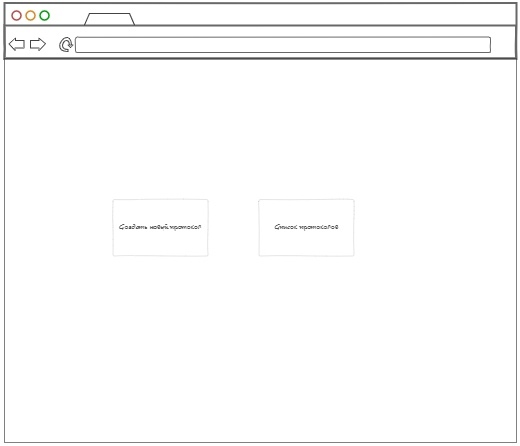
\includegraphics[width=13.20cm,height=11.20cm]{media/image1.ipeg}
	\end{figure}
	
	\begin{center}Рисунок 1 - Макет главной страницы.\end{center}
	
	\begin{figure}[h]
		\centering
		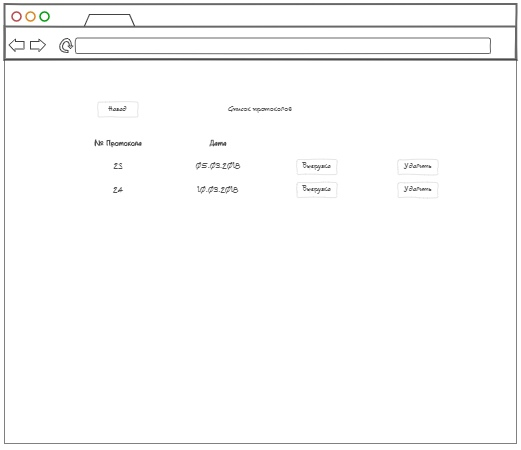
\includegraphics[width=13.20cm,height=11.20cm]{media/image2.ipeg}
	\end{figure}
	
	\begin{center}Рисунок 2 - Макет страницы со списком имеющихся протоколов.\end{center}
	
	\begin{figure}[h]
		\centering
		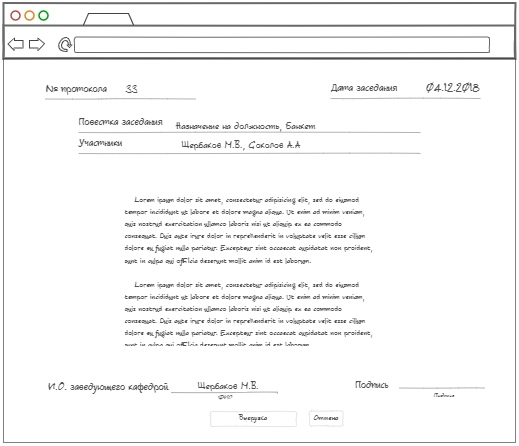
\includegraphics[width=13.20cm,height=11.20cm]{media/image3.ipeg}
	\end{figure}
	
	\begin{center}Рисунок 3 – Макет страницы просмотра имеющегося протокола.\end{center}
	
	\begin{figure}[h]
		\centering
		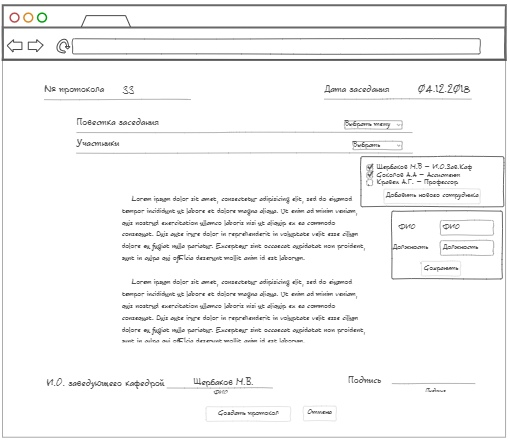
\includegraphics[width=13.20cm,height=11.20cm]{media/image4.ipeg}
	\end{figure}
	
	\begin{center}Рисунок 4 – Макет страницы создания нового протокола (возможно создание участников через саму страницу)\end{center}
	
	\begin{figure}[h]
		\centering
		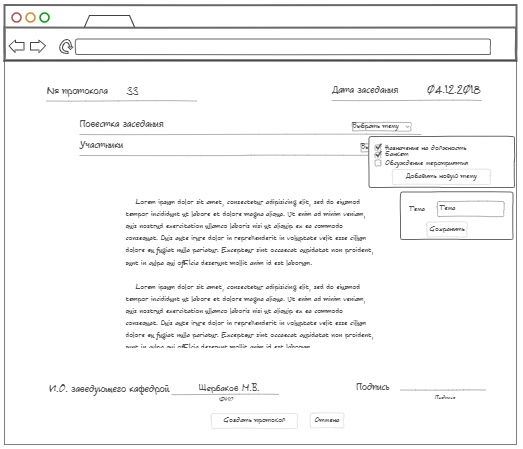
\includegraphics[width=13.20cm,height=11.20cm]{media/image5.ipeg}
	\end{figure}
	
	\begin{center}Рисунок 5 – Макет страницы создания нового протокола (возможно создание тем заседаний через страницу)\end{center}
	
\end{document}